%%%%%%%%%%%%%%%%%%%%%%%%%%%%%%%%%%%%%%%%%%%%%%%%%%%
%% P3: Phenomenology of Particle Physics                         
%%
%% Author:  André Rubbia                   		 
%%
%% Figure 13.6 Forward ($\cos\theta>0$) and backward ($\cos\theta<0$) scattering.
%%
%% This work is licensed under the Creative Commons Attribution 4.0 International License. 
%% To view a copy of this license, visit http://creativecommons.org/licenses/by/4.0/ or 
%% send a letter to Creative Commons, PO Box 1866, Mountain View, CA 94042, USA.
%%
%%%%%%%%%%%%%%%%%%%%%%%%%%%%%%%%%%%%%%%%%%%%%%%%%%%

\documentclass[a4paper,10pt]{article}

\usepackage[T1]{fontenc}
\usepackage[utf8]{inputenc}
\usepackage{lmodern}
\usepackage[labelfont=bf]{caption}
\usepackage{upgreek}

\usepackage{tikz}
\usepackage{pgfplots}
\pgfplotsset{compat=1.17}
\usepgfplotslibrary{ternary}
\usepgfplotslibrary{fillbetween}
\usepgfplotslibrary{external}

\usepackage{braket}

\def\d{\mathrm{d}}

\begin{document}

%%%%%%%%%%%%%%%%% FIGURE %%%%%%%%%%%%%%%%%%%%%%%%%%%%%%%%%%
\begin{figure}[htb]
\begin{center}
\fbox{
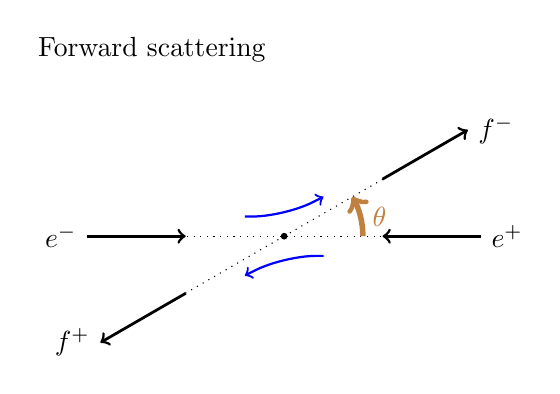
\begin{tikzpicture}[scale=0.5]
\draw[dotted] (-5,0)  -- (0,0);
\draw[dotted] (5,0)  -- (0,0);
\draw[dotted] (0,0) -- +(30:4);
\draw[dotted] (0,0) -- +(-150:4);
\draw[brown,thick,->,line width=2pt] (2,0) arc [radius=2, start angle =0, end angle=30];
\draw[brown] (2,0.5) node[right] {$\theta$};
\draw[->,line width=1pt] (-5,0)  node[left] {$e^-$} -- (-2.5,0);
\draw[->,line width=1pt] (5,0)  node[right] {$e^+$} -- (2.5,0);
\draw[->,line width=1pt] (2.5,1.45)  -- +(30:2.5) node[right] {$f^-$};
\draw[->,line width=1pt] (-2.5,-1.45)  -- +(-150:2.5) node[left] {$f^+$};
\filldraw [black] (0,0) circle (2pt);
\draw[->,thick, blue,rounded corners=4mm ] (-1,0.5) -- (0,0.5) -- (1,1);
\draw[->,thick, blue,rounded corners=4mm ] (1,-0.5) -- (0,-0.5) -- (-1,-1);
\draw[] (-6.5,4.75) node[right] {Forward scattering};
\end{tikzpicture}
}
~\vspace{1cm}\\
\fbox{
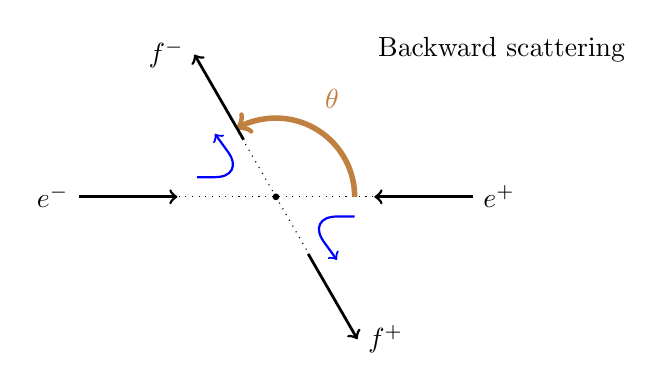
\begin{tikzpicture}[scale=0.5]
\draw[dotted] (-5,0)  -- (0,0);
\draw[dotted] (5,0)  -- (0,0);
\draw[dotted] (0,0) -- +(120:4);
\draw[dotted] (0,0) -- +(-60:4);
\draw[brown,thick,->,line width=2pt] (2,0) arc [radius=2, start angle =0, end angle=120];
\draw[brown] (1,2.5) node[right] {$\theta$};
\draw[->,line width=1pt] (-5,0)  node[left] {$e^-$} -- (-2.5,0);
\draw[->,line width=1pt] (5,0)  node[right] {$e^+$} -- (2.5,0);
\draw[->,line width=1pt] (-0.82,1.45)  -- +(120:2.5) node[left] {$f^-$};
\draw[->,line width=1pt] (0.82,-1.45)  -- +(-60:2.5) node[right] {$f^+$};
\filldraw [black] (0,0) circle (2pt);
\draw[] (2.35,3.75) node[right] {Backward scattering};
\draw[->,thick, blue,rounded corners=4mm ] (-2,0.5) -- (-0.75,0.5) -- (-1.55,1.6);
\draw[->,thick, blue,rounded corners=4mm ] (2,-0.5) -- (0.75,-0.5) -- (1.55,-1.6);
\end{tikzpicture}
}
\end{center}
\caption{Forward ($\cos\theta>0$) and backward ($\cos\theta<0$) scattering.}
\end{figure}
%%%%%%%%%%%%%%%%% END FIGURE %%%%%%%%%%%%%%%%%%%%%%%%%%%%%%
%

\end{document}
